% Automaton corresponding to the formula phi = exists P. (Sing(P) and not P
% \subseteq X)

\documentclass{standalone}

\usepackage{pgf}
\usepackage{tikz}
\usepackage{amssymb}
\usetikzlibrary{arrows,automata}
\usepackage[latin1]{inputenc}
\usepackage{makecell}
\begin{document}
%\begin{figure}
% \begin{center}
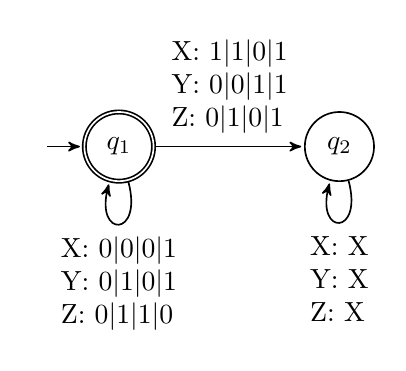
\begin{tikzpicture}[->,>=stealth',shorten >=1pt,auto,node distance=2.8cm,
                    semithick,initial text={}]
  \tikzstyle{every state}=[fill=none,draw=black,text=black]

  \node[initial,state,accepting] (A)                    {$q_1$};
  \node[state]         (B) [right of=A]       {$q_2$};

  \path (A) edge [loop below] node 
  {\makecell[l]{X: 0\textbar0\textbar0\textbar1\\
  				Y: 0\textbar1\textbar0\textbar1\\
  				Z: 0\textbar1\textbar1\textbar0}} (A)
  			edge  node 
  {\makecell[l]{X: 1\textbar1\textbar0\textbar1\\
  				Y: 0\textbar0\textbar1\textbar1\\
  				Z: 0\textbar1\textbar0\textbar1}} (B)
  	    (B) edge [loop below] node {\makecell[l]{X: X\\Y: X\\Z: X}} (B);
        
\end{tikzpicture}
\end{document}